\section{问题四的建模与求解}
\label{sec:problem4}

问题四要求在同一份榜单数据上完成三件相互衔接的工作：把窗口内的能力提升拆分为规模扩张与非规模技术进步两个通道；在算力增长放缓的情景下预测未来前沿并给出不确定性；建立交叉熵损失与多维基准得分之间的映射。三者的顺序由数据条件决定：归因只能在给出参数量标注的投榜记录上进行，故样本口径须先行固定；预测要把损失尺度上的标度律换算到得分尺度，故桥接必须前置，其误差也要一并进入预测区间。

\subsection{样本口径与两个核心定义}
\label{subsec:q4-scope}

本节分析的总体是 Open LLM Leaderboard 上的投榜模型（leaderboard submissions），而非开源模型的总体\citep{beeching2023leaderboard}。投榜由模型方自行决定，进入榜单的记录在参数量分布与评测版本上不构成随机抽样，榜单自身在测试集污染与版本切换上的已知问题也会一并进入数据\citep{fourrier2024leaderboard}，故下文的结论以该投榜样本为范围，不外推到开源模型总体。

样本按三项口径固定。其一为开源筛选，只保留公开权重并给出参数量标注的记录；其二为模型类型，按元数据中的类型字段区分预训练模型（pretrained）与对话微调模型（chat/finetuned），分组分解针对这两族；其三为时间轴，按提交日期把记录归入月份。参数量与类型标注由 C4 元数据经模型名称规范化连接得到，无法匹配的记录按缺失处理；该连接把两个附件的记录视为同一模型，是全节的前提。窗口取 2024 年 6 月至 2025 年 3 月，共 278 天，约合 9.1 个月，覆盖 10 个月度锚点，可用的分解样本为 4561 行。表~\ref{tab:q4-scope}汇总了这些固定设定。

\begin{table}[H]
  \centering
  \caption{问题四的固定口径与关键设定}
  \label{tab:q4-scope}
  \begin{tabular}{@{}ll@{}}
    \toprule
    项 & 设定 \\
    \midrule
    样本总体 & Open LLM Leaderboard 投榜模型（非开源模型总体） \\
    窗口 & 2024 年 6 月--2025 年 3 月，278 天（约 9.1 个月，10 个月度锚点） \\
    分解样本 & 4561 行 \\
    综合能力 $S$ & C1 的 Average 字段，六项基准等权平均（分） \\
    前沿 & 每月 $S$ 的 0.90 分位，记作 $S_{q90}$ \\
    规模通道口径 & 仅参数量，在全样本上估计 \\
    预测视界 & 12 个月（主要视界；24 个月一并报告，仅作附带讨论） \\
    \bottomrule
  \end{tabular}
\end{table}

综合能力 $S$ 取 C1 的 Average 字段，即 IFEval、BBH、MATH Level 5、GPQA、MUSR 与 MMLU-PRO 六项基准的等权平均，沿用榜单现有口径，以避免引入无法在数据内检验的权重。前沿（frontier）定义为每月 $S$ 的 0.90 分位，记作 $S_{q90}$；相应地，每月的参数量 0.90 分位记作 $N_{q90}$。取分位而非最大值，是因为按月样本量在 173 至 868 之间波动，极值对个别记录过于敏感。规模通道仅以参数量度量，在全样本上估计；训练 token 数与算力字段缺失较多，不进入主口径，其作用见第~\ref{subsec:q4-group}~小节。本节的技术路线见图~\ref{fig:q4-framework}。

问题四的技术路线。上方固定榜单窗口与样本，左侧由逐模型得分与参数量、分解规格进入通道分解，再作端点定义与函数规格的双重扰动；通道分解刻画规模贡献并扣除该贡献以得到技术通道。右侧将月度能力前沿、问题二参数与桥接及通道分解结果用于情景预测，并与纯趋势基线对照。

\begin{figure}[H]
  \centering
  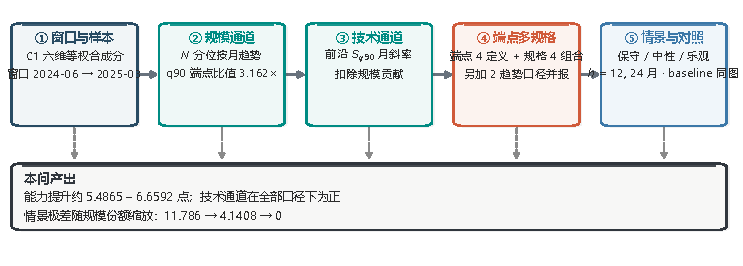
\includegraphics[width=0.98\linewidth]{figures/fig_framework_q4.pdf}
  \caption{能力变化分解与前沿情景预测流程}
  \label{fig:q4-framework}
\end{figure}

\subsection{归因模型的设定与识别性}
\label{subsec:q4-model}

设模型 $i$ 在月份 $t(i)$ 的综合得分为 $S_i$，本节采用的加性分解为
\begin{equation}
  S_i = f(N_i) + \tau_{t(i)} + \varepsilon_i,
  \label{eq:q4-decomp}
\end{equation}
其中 $f(N)$ 为规模通道函数，$\tau_t$ 为第 $t$ 月的技术通道效应，$\varepsilon$ 为残差。两通道在窗口内的贡献分别定义为规模项在末月与首月的期望之差，以及技术项在末月与首月之差：
\begin{equation}
  \Delta_{\text{scale}} = \mathbb{E}\!\left[f(N)\mid \text{末月}\right] - \mathbb{E}\!\left[f(N)\mid \text{首月}\right],
  \qquad
  \Delta_{\text{tech}} = \tau_{\text{末月}} - \tau_{\text{首月}}.
  \label{eq:q4-contrib}
\end{equation}

$f(N)$ 的主口径不是 $\log N$ 的线性项，而是 $\log N$ 的十分位虚拟变量。该选择针对窗口内规模分布的形状变化：如第~\ref{subsec:q4-trend}~小节所示，高分段的参数量在下降而中位数基本不动，十分位虚拟变量把这一形变吸收进各档的截距，不跨分布外推斜率。$\tau_t$ 取月度固定效应，每月一个自由参数，首月归一化为零，它因此吸收了规模项之外的全部月度共同变动：数据质量的改善、语料治理与训练工程的经验积累、评测模板的调整，以及模型对榜单基准的过拟合\citep{fourrier2024leaderboard}。本文把该通道统一表述为\textbf{非规模技术/数据工程综合进步}，不解释为架构或算法的进步——该通道无法把上述成分彼此分离，窗口内也没有外生变量可供识别。

模型的可分性依赖于时间与规模不共线，这一点在本数据上成立。时间与 $\log N$ 的秩相关为 $-0.0615$，近乎正交；$S$ 与 $\log N$ 的秩相关为 $+0.6352$，规模项确有解释力。把样本按参数量分成四个档位后分别估计月度效应，四档内 $\tau$ 均显著为正，其中 4--10B 档内时间与得分的秩相关为 $0.3125$，10--30B 档为 $0.4827$。档内时间与规模已不共线，档间差异由十分位虚拟变量承担，故两通道可以分开估计。

分解的代数性质也在数值上核验过。式~\eqref{eq:q4-decomp} 为加性结构，两因子的 Shapley 值与式~\eqref{eq:q4-contrib} 恒等，没有交互项需要估计；四种函数规格与四种端点定义下，两通道点数之和均等于合计提升，份额之和恒为 1。份额因此可直接由点数读出，其适用边界见下文。规模通道的写法与经典标度律并不等同：后者描述损失随规模的变化\citep{kaplan2020,hoffmann2022}，以分布形状稳定为前提\citep{bahri2024}，本节只估计规模项在观测分布上的取值。

\subsection{分解结果与口径敏感性}
\label{subsec:q4-perturb}

主口径（$\log N$ 十分位、月度固定效应、单末月读数）给出规模通道 1.7175 分、技术通道 4.9069 分，合计 6.6244 分。按月内重抽模型的自助区间（重抽 2000 次）为：规模点数 $[0.1314,\ 2.9714]$，技术点数 $[3.7183,\ 6.5857]$。技术通道的点数在重抽样下远离零，规模通道虽为正，其份额并不稳定。

自助区间只重抽模型，不重抽口径选择，在结构上覆盖不了换一个末端定义或换一种 $f(N)$ 规格的摆动，两类扰动的结果列于表~\ref{tab:q4-perturb}。

\begin{table}[H]
  \centering
  \caption{通道分解对端点定义与函数规格的敏感性（单位：分；份额无量纲）。端点扰动的四个口径分别覆盖 4561、1477、2345 与 4219 行。}
  \label{tab:q4-perturb}
  \begin{tabular}{@{}lrrrr@{}}
    \toprule
    通道口径 & 规模通道 & 技术通道 & 合计 & 规模份额 \\
    \midrule
    主口径：$\log N$ 十分位 $\times$ 月度 $\times$ 单末月 & 1.7175 & 4.9069 & 6.6244 & $+0.2593$ \\
    \midrule
    端点：首月对末两月合并 & 1.2040 & 5.4438 & 6.6477 & $+0.1811$ \\
    端点：首月对末三月合并 & $-0.1547$ & 5.6412 & 5.4865 & $-0.0282$ \\
    端点：去掉末月 & 1.4685 & 5.1908 & 6.6592 & $+0.2205$ \\
    \midrule
    规格：线性 $\log N$，月度 & $-1.8730$ & 8.4975 & 6.6244 & $-0.2827$ \\
    规格：$\log N$ 十分位，季度 & 0.4567 & 5.0298 & 5.4865 & $+0.0832$ \\
    规格：线性 $\log N$，季度 & $-2.7280$ & 8.2145 & 5.4865 & $-0.4972$ \\
    \midrule
    趋势法：$\log N$ 十分位（十个月斜率） & 0.5175 & 5.1640 & 5.6815 & $+0.0911$ \\
    趋势法：线性 $\log N$（十个月斜率） & $-3.0343$ & 8.7158 & 5.6815 & $-0.5341$ \\
    \bottomrule
  \end{tabular}
\end{table}

规格扰动会使规模通道的符号翻转。线性 $\log N$ 规格给出规模通道 $-1.8730$ 分、技术通道 8.4975 分，规模份额 $-0.2827$；把月度固定效应换成季度后，线性规格的规模份额进一步降至 $-0.4972$。该结果不是计算缺陷，而是线性规格的必然产物：窗口内高分段的规模在下降，当 $f(N)$ 的斜率被约束为正时，规模项的末月与首月期望之差必然为负。十分位规格不做这一外推，故给出正号的规模贡献。两种规格的读数差别不影响方向判断，故一并列出。

端点扰动给出同类的结论。把末月的定义由单月改为末两月合并、末三月合并或去掉末月，规模份额依次为 $+0.2593$、$+0.1811$、$-0.0282$、$+0.2205$，极差 $0.2875$，并发生一次符号翻转，该极差已大于主口径的规模份额 $0.2593$ 本身。技术份额在四种端点定义下分别为 $0.7407$、$0.8189$、$1.0282$、$0.7795$，方向始终为正；各口径的两通道贡献见图~\ref{fig:q4-channel}。

各口径下的通道贡献分解与子组份额。(a) 横轴为能力提升（C1 分值），每个口径一条堆叠条，深色为技术/数据工程通道、浅色为规模通道，菱形为合计提升，四种端点/规格算法给出的极差为 5.4865--6.6592 分，规模通道的条在若干口径下伸向负半轴。(b) 对话微调组的规模通道份额及其 95\% 自助区间，竖直虚线为份额等于 1 的位置；预训练组的合计提升为负，其份额的分母为负，该组的份额与区间不在图中给出。

\begin{figure}[H]
  \centering
  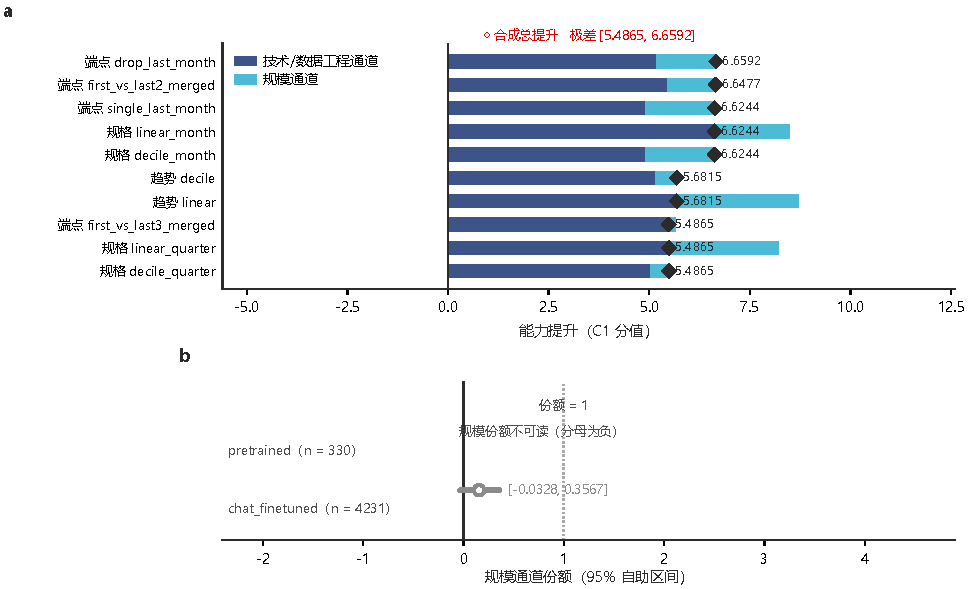
\includegraphics[width=0.98\linewidth]{figures/fig_q4_channel_decomposition.pdf}
  \caption{不同口径的通道贡献及对话微调组的规模份额}
  \label{fig:q4-channel}
\end{figure}

两类扰动的共同含义是：通道方向稳健，具体比例并不稳健。技术通道在表~\ref{tab:q4-perturb} 的九种口径下全部为正（最低 $0.7407$、最高 $1.5341$），规模通道的份额则随规格与端点变号。主口径的自助区间 $[0.0223,\ 0.4019]$ 不含零，但它只测「换一批模型」，不测「换一个末端定义」，后者给出的极差已超过主口径的规模份额，故该区间不含零不构成规模贡献显著为正的证据。上述扰动只支持通道方向的结论，不支持任何具体比例。

合计提升在四种端点/规格算法下的极差为 5.4865--6.6592 分。这一区间是这四种算法的极差，而不是全部方法的极差：趋势法只用九个月的 drop-last 变体给出 5.3581 分，略低于下界，相差约 0.13 分，量级上不改变任何结论。

\subsection{趋势法读数与规模—前沿的同期走势}
\label{subsec:q4-trend}

端点法只用窗口两端的读数，会把月间波动压缩成一个差值；趋势法改用全部十个月的斜率定义通道贡献，是本节主结论的实际依据。两通道的月斜率分别为 $+0.05750$ 与 $+0.57377$（均为分/月），后者约为前者的 9.98 倍。按九个月区间累积，规模通道贡献 0.5175 分、技术通道 5.1640 分，合计 5.6815 分。规模份额为 $+0.0911$，按月分层重抽 1000 次所得的自助 95\% 区间为 $[-0.1942,\ +0.2258]$，含零。

关键量是斜率比而非份额：技术通道的月斜率比规模通道高一个数量级，规模份额很小且其区间含零。两项读数合起来给出本节的主结论：窗口内的能力提升由非规模技术/数据工程综合进步主导，规模通道的贡献与零不可区分。合计 5.6815 分落在端点法的区间之内，两种口径相互印证。

同期规模与前沿的走势方向相反，这一对比是理解上述结果的前提，见图~\ref{fig:q4-scale-frontier}。前沿 $S_{q90}$ 由首月的 25.9201 分升至末月的 41.3875 分，对月份做线性拟合的斜率为 $+1.5333$ 分/月。参数量分位则在下降：$N_{q90}$ 由 46.703B 降至 14.770B，端点比值为 3.162，即缩至首月的 $1/3.162$；$\log_{10} N_{q90}$ 的月斜率为 $-0.06281$，窗口内累计（9 个月度间隔）$-0.5653$ dex，按该斜率换算的隐含比值为 $10^{0.5653} = 3.675$。两个比值描述的不是同一口径，其差别来自 $N_{q90}$ 逐月路径的非单调——2024 年 8 月一度回升至 70.554B，其后稳定在 14.77B 附近，斜率不经过端点。

规模与前沿的同期走势。(a) 纵轴为模型参数量（十亿，对数刻度），细线为每月参数量分布的 0.10、0.50 与 0.90 分位及最大值，其中 0.90 分位由 46.703B 降至 14.770B，端点比值为 3.162。(b) 纵轴为前沿能力 $S_{q90}$（分），红色虚线为线性拟合，斜率 $+1.5333$ 分/月，末月读数为 41.3875 分。

\begin{figure}[H]
  \centering
  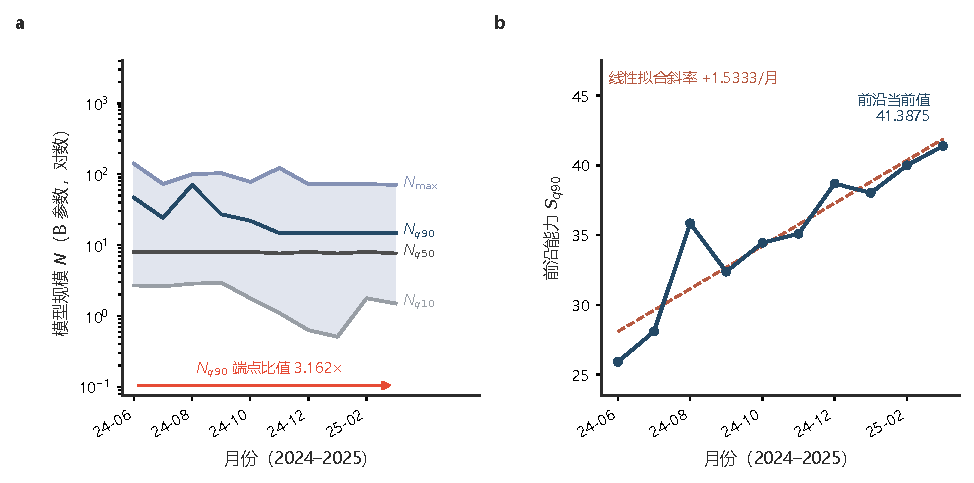
\includegraphics[width=0.98\linewidth]{figures/fig_q4_scale_vs_frontier.pdf}
  \caption{模型参数量分布与能力前沿的同期走势}
  \label{fig:q4-scale-frontier}
\end{figure}

下降集中在高分段。$\log_{10} N$ 中位数的月斜率仅为 $-0.00209$，即中位规模在整个窗口内基本不动；0.10 分位的月斜率为 $-0.05714$，0.90 分位为 $-0.06281$。前沿变强的同时，站上前沿的模型在变小；这与趋势法的分解结果一致——若能力提升主要来自规模扩张，$N_{q90}$ 不应下降。前沿推进的来源可在语料工程一侧找到对应：固定算力下改变数据选择与配比，其收益可以超过单纯扩大规模\citep{sorscher2022,goyal2024filtering}；窗口内投榜模型的中位规模基本不变，能力差异更多来自数据与训练过程\citep{dubey2024llama3}。

\subsection{子组分解与规模通道的度量口径}
\label{subsec:q4-group}

题目要求区分预训练与对话/微调两类模型，分组结果列于表~\ref{tab:q4-group}。

\begin{table}[H]
  \centering
  \caption{按模型类型的子组分解（主口径，单位：分；份额无量纲）。预训练组的合计提升为负，其份额失去解释力，故只报绝对点数与方向。}
  \label{tab:q4-group}
  \begin{tabular}{@{}lrrrrl@{}}
    \toprule
    子组 & $n$ & 规模通道 & 技术通道 & 合计 & 规模份额（95\% 自助区间） \\
    \midrule
    对话微调 & 4231 & 1.0921 & 5.9356 & $+7.0278$ & 0.1554 $[-0.0328,\ 0.3567]$ \\
    预训练 & 330 & $-5.9745$ & 2.3955 & $-3.5789$ & 不可读（分母为负） \\
    \bottomrule
  \end{tabular}
\end{table}

对话微调组（$n=4231$）合计提升 $+7.0278$ 分，规模通道 1.0921 分、技术通道 5.9356 分，规模份额 $0.1554$，其自助 95\% 区间 $[-0.0328,\ 0.3567]$ 含零，故该组的规模贡献不能被认定为显著为正。预训练组（$n=330$）给出方向相反的读数：合计 $-3.5789$ 分，其中规模通道 $-5.9745$ 分、技术通道 $+2.3955$ 分。该组在本窗口内能力是回落的，而非提升的。回落本身是可报告的读数，但其份额不可解释：份额是两个通道之比，分母为负时该比值的符号与量级都失去意义，故对该组只报告绝对点数与方向。预训练组仅占全样本的 7.2\%，分组估计的精度低于全体，两组的结论也不能互相推广：对话微调组的正提升不能推断预训练模型在进步，预训练组的回落也不能推断开源前沿在退步。

规模通道的度量口径需要一个对照：主口径只取参数量，另一口径同时纳入参数量、训练 token 数与算力。在同时给出这三项元数据的 66 个模型子集上，仅取参数量的口径给出规模通道 $-3.1404$ 分、技术通道 $-1.4083$ 分，三项并取的口径给出规模通道 $-3.3855$ 分、技术通道 $-1.1631$ 分。两者的规模点数相差 $+0.2451$ 分，技术点数相差 $-0.2451$ 分，精确抵消。

这一对照支持的是机制，而不是方向。省略算力与数据量会在两个通道之间重分配解释力，重分配量约 0.25 分，总量不变；但该子集的合计提升为 $-4.5487$ 分，为负值，两个通道的份额都不可读，点数比较的符号关系不能用来判定偏误方向。该子集的末期（2025 年第一季度）只有 3 个模型，中位 $\log_{10} N$ 降至 0.180、平均得分降至 7.765，其负的合计提升是端点抽样的产物；该子集中预训练模型的占比又远高于全样本，两者并非同一总体。因此这里的 0.2451 分只作机制的量级参考，不构成对全样本口径的修正。

\subsection{从损失到得分的桥接与误差传播}
\label{subsec:q4-bridge}

预测需要在损失尺度上进行，而问题二的标度律以验证集交叉熵损失为因变量、前沿以基准得分为尺度，两者的换算关系必须由实际观测拟合，不能假定。桥接数据（C6，75 行）同时给出验证集损失与榜单得分，按可比性分为 High 与 Medium 两层，以 $3:1$ 的层级权重拟合
\begin{equation}
  \text{LB\_Average} = 62.7406 - 22.393 \times \text{Val\_Loss},
  \label{eq:q4-bridge}
\end{equation}
验证集损失与榜单得分呈单调递减关系（斜率 $-22.393$，95\% 置信区间 $[-44.481,\ -7.8308]$），均方根误差为 10.9842 分，各项列于表~\ref{tab:q4-bridge}。

\begin{table}[H]
  \centering
  \caption{损失到得分的桥接拟合及其分层核验（单位：分）。秩相关为斯皮尔曼系数。}
  \label{tab:q4-bridge}
  \begin{tabular}{@{}lrl@{}}
    \toprule
    量 & 值 & 备注 \\
    \midrule
    截距 & 62.7406 & 式~\eqref{eq:q4-bridge} \\
    斜率 & $-22.393$ & 95\% 置信区间 $[-44.481,\ -7.8308]$ \\
    均方根误差 & 10.9842 & 与得分本身同量级 \\
    映射误差 $\sigma$ & 10.1726 & 作为独立随机项并入预测 \\
    桥接样本 & 75 行 & High 层 7 行、Medium 层 68 行，权重 $3:1$ \\
    High 层秩相关 & $-0.6071$ & $p$ 值 $0.148$ \\
    Medium 层秩相关 & $-0.5087$ & $p$ 值 $9.4\times10^{-6}$ \\
    \bottomrule
  \end{tabular}
\end{table}

High 层只有 7 个样本，其秩相关 $-0.6071$（$p$ 值 $0.148$）与式~\eqref{eq:q4-bridge} 方向一致但不显著；Medium 层 68 个样本的秩相关为 $-0.5087$（$p$ 值 $9.4\times10^{-6}$）。样本量是 High 层不显著的原因，不能据此认为该层质量更差。残差标准差 10.1726 分与得分本身同一量级，这是 9.1 个月窗口与 75 行桥接样本所能给出的精度；该误差被作为独立随机项并入蒙特卡洛预测，区间因此偏宽，而宽度是数据条件的结果，不是算法上的取舍。桥接也不引入循环论证：用于拟合的损失值全部来自技术报告与训练日志，不含由标度律反推的估计行，式~\eqref{eq:q4-bridge} 的输入不包含问题二的结论。

\subsection{前沿预测与基线对照}
\label{subsec:q4-forecast}

预测以 $S_{q90}$ 为对象。做法是把前沿自身的月斜率按规模份额拆入两个通道，得到技术通道 1.1358 分/月与规模通道 0.3975 分/月（合计 $+1.5333$ 分/月），再对两个通道分别施加情景假设：规模通道随算力增速缩放，技术通道按年衰减率衰减。三个情景的设定为保守（算力 1.5 倍/年，技术衰减 0.50）、中性（2.5 倍/年，0.75）与乐观（4.0 倍/年，1.00）。技术趋势斜率、桥接映射误差 $\sigma=10.1726$ 与桥接斜率的不确定性 $[-44.481,\ -7.8308]$ 三类来源同时抽取，蒙特卡洛重复 4000 次。表~\ref{tab:q4-forecast}给出 12 个月视界的结果，并按同口径列出纯趋势基线 M0a（$q90_t = a + b\,t$，斜率 1.5333 分/月）的对应读数。

\begin{table}[H]
  \centering
  \caption{12 个月视界的前沿预测与纯趋势基线的同口径对照（单位：分）。当前前沿为 41.3875 分；预声明的预测判据取中性行的 80\% 区间下界（43.268 分）。}
  \label{tab:q4-forecast}
  \begin{tabular}{@{}lrrrr@{}}
    \toprule
    口径 & 中位数 & 80\% 区间 & 95\% 区间 & 95\% 宽度 \\
    \midrule
    保守（1.5 倍/年，衰减 0.50） & 50.249 & $[37.246,\ 63.701]$ & $[30.237,\ 71.120]$ & 40.883 \\
    中性（2.5 倍/年，衰减 0.75） & 56.330 & $[43.268,\ 69.699]$ & $[35.513,\ 77.449]$ & 41.935 \\
    乐观（4.0 倍/年，衰减 1.00） & 62.035 & $[49.189,\ 75.672]$ & $[41.683,\ 82.867]$ & 41.184 \\
    基线 M0a（纯趋势，不分解） & 60.290 & $[56.448,\ 64.131]$ & $[54.415,\ 66.165]$ & 11.750 \\
    \bottomrule
  \end{tabular}
\end{table}

中性情景下 12 个月的前沿中位数为 56.330 分，80\% 区间 $[43.268,\ 69.699]$，95\% 宽度 41.935 分，约等于当前前沿值本身；基线在同一视界上给出 60.290 分，80\% 区间 $[56.448,\ 64.131]$，95\% 宽度 11.750 分。两者相比，主方法的点值低约 6.6\%，95\% 区间宽约 3.6 倍。差异来自结构而非随机性：主方法对技术趋势施加了情景衰减，基线不做衰减，且基线不承担桥接环节的映射误差。

预测使用的标度律参数承接问题二，其中质量指数的反解依赖半合成网格（附件 B6--B8），该部分带补充分析的性质，不构成直接实验观测；该标度律的数据量指数可跨源共享这一前提已在问题二中单独检验并判为不成立（见第~\ref{sec:problem2}~节），此处按承重前提使用，其条件性一并继承。该依赖只影响情景读数的具体幅度。

预声明的预测判据为：中性情景下 12 个月的 80\% 区间下界高于当前前沿值。实测下界为 43.268 分，高于 41.387 分，裕度 1.881 分。该判据的执行过程有一次次序需要说明。首轮实现把均值层面的技术通道月斜率 0.4675 分直接加到 0.90 分位的前沿水平上，两端对象不一致，使预测系统性偏低，首轮下界为 32.276 分，判据不通过；修正为用前沿自身的斜率按规模份额拆通道之后，下界升至 43.268 分。判据文字自始未改，但缺陷是在看到首轮不通过之后才被发现的，这限制了该判据作为独立验证的分量。

基线也满足同一判据：其 80\% 区间下界为 56.448 分，高于当前前沿，就该判据而言主方法不构成对基线的优势。主方法的价值在于给出可按通道拆解、并随算力情景变化的区间，代价是区间更宽、点值更低。

本节以 12 个月为主要视界，24 个月仅作附带讨论。乐观情景的 24 个月中位数为 94.118 分，逼近得分 0--100 的上界，其 95\% 宽度 29.236 分反而窄于同情景 12 个月的 41.184 分；这一收窄是截断到上界造成的，不是精度的提高；得分上界的饱和形态在 9.1 个月的窗口内无法检验，24 个月的读数仅在上述限制下具有参考意义。评测指标的取值方式本身会塑造所观察到的能力形态，在指标存在截断或分辨率受限时尤其如此\citep{schaeffer2023}。

情景极差随规模份额严格缩放，见图~\ref{fig:q4-forecast}。表~\ref{tab:q4-forecast}中的三个情景对应主口径的规模份额 $0.2593$，其极差为 11.786 分；若改用趋势法的份额 $0.0911$，极差按同一比例降至 4.1408 分，约为中性中位数的 7.4\%；份额趋零时极差亦趋零。算力增长放缓对开源前沿的短期预测影响很小，因为前沿的推进本就不依靠规模扩张\citep{muennighoff2023}。

前沿预测与情景缩放。(a) 横轴为 C1 分值，各行对应一个情景与预测视界；三个情景各给出 12 个月与 24 个月两个视界的中位数（空心圆）、80\% 区间（粗段）与 95\% 区间（细线），灰色一行为纯趋势基线 M0a 的 12 个月读数，红色竖线为当前前沿 41.3875 分。(b) 横轴为规模通道份额，纵轴为 12 个月视界上的三情景极差；份额为 0.2593、0.0911 与 0 时，极差分别为 11.79、4.141 与 0 分。

\begin{figure}[H]
  \centering
  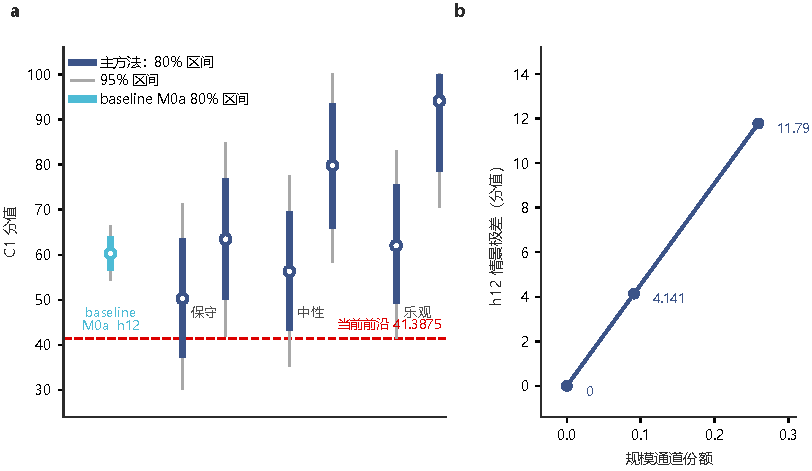
\includegraphics[width=0.98\linewidth]{figures/fig_q4_forecast_scenarios.pdf}
  \caption{前沿预测与情景缩放}
  \label{fig:q4-forecast}
\end{figure}

\subsection{基准内部的逐任务聚合}
\label{subsec:q4-c8}

题目要求在给定基准内部给出逐任务的聚合，不能只用汇总表。C8 提供各模型在 BBH 等基准上的逐任务明细：可解析目录 1860 个，另有 4 个文件因同一次导出事故不可解析；得到任务级记录 65137 条，其中 BBH 含 24 个子任务。

聚合口径为：先在每个子任务内对全部模型做 z 标准化，再按模型对子任务取均值。逐任务标准化的必要性在于 24 个子任务的通过率量纲不同，直接相加会让容易的子任务主导排序。按该口径得到 1860 个模型的 z 分数，均值为 $-0.0$、标准差 0.8037。子任务之间的难度落差明显：最难的 5 项为 \path{tracking_shuffled_objects_seven_objects}（0.1743）、\path{tracking_shuffled_objects_five_objects}（0.2033）、\path{geometric_shapes}（0.3285）、\path{tracking_shuffled_objects_three_objects}（0.3298）与 \path{object_counting}（0.3409）；最易的 5 项为 \path{boolean_expressions}（0.7640）、\path{sports_understanding}（0.6801）、\path{hyperbaton}（0.6320）、\path{snarks}（0.6026）与 \path{navigate}（0.5850）。前者的主体是多步状态追踪与计数，后者以单步布尔判断与常识为主，难度排序与推理步数一致。

缺失基准按可比样本子集口径处理：某个模型在某个子任务上没有记录时，该子任务不参与该模型的均值，也不以零填充——零填充在通过率量纲上等同于「全部答错」，会把记录缺失误读为能力低下。该口径保持了同一模型内部各子任务的可比性，代价是不同模型之间的有效子任务集合并不完全相同，故这些 z 分数适用于模型内部的排序，不宜直接跨模型作绝对水平的比较。
